\section{Ferramentas}

As próximas secções introduzem ferramentas utilizadas no projecto, desde bibliotecas ruby e javascript a base de dados.

\subsection{Ruby}

Ruby é uma linguagem de programação intrepertada com suporte para diferentes paradigmas (funcional, orientado a objectos e imperativo). Desde o lançamento em 1995 Ruby tem crescido em comunidade e potencial. O seu criador, Yukihiro Matsumoto, pretendia uma linguagem que qualquer programador pudesse aperciar:

\begingroup
\leftskip4em
\rightskip\leftskip
``Ruby is simple in appearance, but is very complex inside, just like our human body.'' \cite{matz}
\par
\endgroup

Ruby encontra-se actualmente na versão 2.0.0-p195 no entanto o projecto foi desenvolvido na versão \textbf{2.0.0p0}.

\subsubsection{\textit{Global Interpreter Lock}}
\label{sec:gil}

Existem diversos intrepertadores para Ruby sendo os mais importantes \textbf{Matz's Ruby Interpreter (MRI)}, em homenagem ao criador, e \textbf{JRuby}, implementado no topo da Java Virtual Machine. 
A diferença mais relevante entre ambos para este projecto é o \textit{Global Interpreter Lock} (GIL) que existe no MRI. O GIL é uma camada responsável por proteger o intrepertador contra código \textit{non thread-safe}.

A figura~\ref{fig:ruby-gil} apresenta uma comparação entre três versões do Ruby. Na versão 1.8 o intrepertador Ruby possuí apenas uma thread do sistema para execussão. Já na versão 1.9, e também na versão 2 ainda que não seja visível na imagem, várias threads do sistema são alocadas ao intrepertador, o que parece prometer paralelismo de execussão. No entanto em ambos os casos existe a camada do GIL que protegendo contra a execussão de código \textit{non thread-safe} permite que apenas uma thread seja executada de cada vez pelo processador, ou seja, ambas as versões do Ruby correm num core do CPU apenas.
Por outro lado a implementação em JRuby não contém a camada GIL o que abre as portas ao paralelismo das aplicações em Ruby.

\begin{figure}[H]
\centering
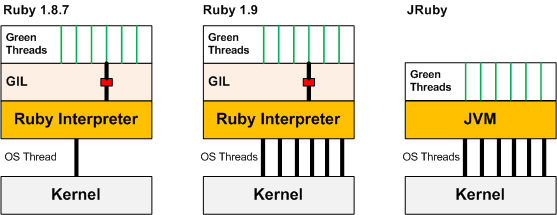
\includegraphics[width=0.9\textwidth]{xruby_gil.png}
\caption{\textit{Global Interpreter Lock}}
\label{fig:ruby-gil}
\end{figure}

Parecendo um cenário desvantajoso para o MRI é de notar que existem soluções para contornar este problema. Se se pensar em processos em vez de threads por procurar-se outros meios de repartir trabalho. Decompondo a aplicação e adicionando meios de comunicação entre processos (Starling, RabbitMQ, outros) consegue-se que multiplos processos da mesma aplicação executem concurrentemente.

\subsubsection{RubyGems}

Pode considerar-se que o projecto é composto por duas aplicações, cliente e servidor. A aplicação servidor, desenvolvida Ruby, encontra-se no formato RubyGem, geralmente denominado por gem. Uma gem é uma biblioteca num formato especifico que pode facilmente se descarregada, instalada e manipulada num sistema que possuia Ruby.\cite{rubygems} O que se pretende com esta preocupação é permitir que a aplicação possa facilmente ser distribuída e desse modo também contribuir para a comunidade Ruby. O formato RubyGem é constituído geralmente pelas seguintes componentes:

\begin{description}%[leftmargin=!,labelwidth=\widthof{\bfseries Código da aplicação }]
\item[Gemspec] Ficheiro que identifica as dependência da gem.
\item[Código da aplicação] Código a executar pela aplicação, encontra-se na pasta \textit{lib}.
\item[Testes] Testes da aplicação. No caso deste projecto os testes são \textbf{RSpec} e encontram-se na pasta \textit{spec}.
\item[Excutáveis] Ficheiros executáveis que são instalados no sistema que podem ser invocados pelo utilizador ou outro software. Encontram-se na pasta \textit{bin}.
\end{description}

\subsubsection{EventMachine}
EventMachine é uma biblioteca para Ruby que implementa \textit{event-drive I/O}. Como se justifica na secção~\ref{sec:gil} Ruby não foi inicialmente concebido para executar concorrentemente e como tal surgem outras alternativas que procuram tirar melhorar o desempenho das aplicações desenvolvidas em Ruby. A biblioteca EventMachine é utilizada para web servers, email, proxies e outros. 

Existem diversas implementações de diferentes protocolos sobre a biblioteca EventMachine. No contexto deste projecto faz-se uso da implementação \textbf{EventMachine Websockets} que fornece um servidor de websockets. Esta biblioteca é a base da componente servidor da aplicação. 

\subsubsection{ActiveRecord}
Esta ferramenta é já parte do cliente.
Active Record é um biblioteca Ruby que establece uma ligação entre classes e tabelas de bases de dados relacionais sem grande configuração. Esta biblioteca uma classe base que quando é extendida establece um mapeamento entre a nova classe e um tabela existente na base de dados. A biblioteca foi desenvolvida inicialmente para a framework Ruby on Rails sendo o base do que se chama models.

É importante referir que o uso desta biblioteca permite que não se escreva SQL de de operações sobre a base de dados à excepção da criação de tabelas sendo esta processo gerado por operações em Ruby.

\subsection{PostgreSQL}

No primeiro esquema conceptual da arquitectura da aplicação planeou-se utilizar SQLite, cada broker teria a sua base de dados e depois haveria sincronização entre todos. 

A primeira abordagem além de complexa não explora o \textbf{controlo de concurrência} que grande parte das base de dados oferece como garantido. Como tal a nova abordagem passa por centralizar a base de dados e todos os servidores trabalham sobre a mesma conseguindo-se sincronização e controlo de concurrência.

\subsection{JQuery}

jQuery é uma biblioteca JavaScript que facilita a manipulação de HTML, eventos, animação, Ajax, entre outros, contendo uma API transversal aos browsers.
Esta bibliteca é base do desenvolvimento do cliente uma vez que facilita muitas operações no código do cliente.


